\chapter{System Design}
\label{sec:systemDesign}
Zur Erfüllung der im vorherigen Kapitel dargestellten Use-Cases wurde sich auf ein System mit drei Teilen geeinigt. Zunächst benötigt das System ein Gerät zur Aufzeichnung der OBD-Daten. Da dieses Gerät der Bequemlichkeit wegen im Fahrzeug verbleiben soll und vermutlich wenig Ressourcen besitzt, verfügt das geplante System zusätzlich noch über ein Backend welches die aufgezeichneten Daten langfristig speichern und auswerten soll. Zusätzlich erfolgt noch eine Anbindung einer Smartphone-App, welche die Fahrzeug-Daten während der Fahrt veranschaulichen soll. Der Vorteil dieser Lösung liegt in der Möglichkeit, die Software der drei Komponenten OBD-Dongle, App und Backend paralell entwickeln zu können. Somit ergibt sich das in Abbildung \ref{fig:SysArch} dargestellte System.
\begin{figure}[h]
  \begin{center}
    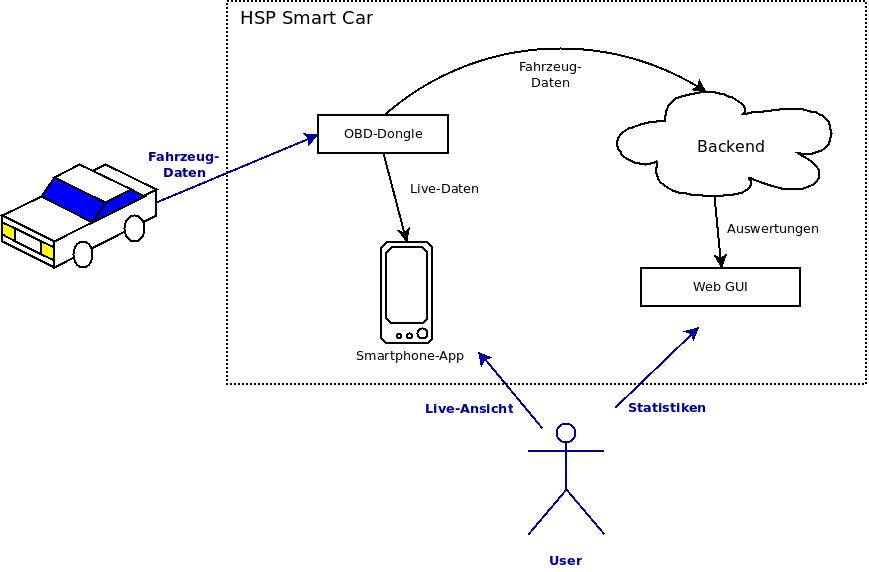
\includegraphics[height=7cm,keepaspectratio]{./img/SysArch}
    \caption{Darstellung des Systems im Kontext}
    \label{fig:SysArch}
  \end{center}
\end{figure}



\section{App}
Um die Fahrzeugdaten während der Fahrt analysieren zu können, sowie auch ein einfacher Weg die Daten vom OBD-Dongle ins Backend zu übertragen, wurde eine plattformübergreifende Smartphone-App erstellt. Die App ist sowohl für Android, IOS als auch Windows verfügbar. Dafür wurde das für mobile Anwendungen konzipierte Framework Apache Cordova verwendet. Dieses Entwicklung-Framework verwendet die standard-Web-Technologien HTML5, CSS3 und JavaScript für die Cross-Plattform-Entwicklung. Die Bibliothek visualisiert die Anwendung mittels, die von den einzelnen Plattformen bereitgestellten, \enquote{WebViews}. Diese zeigen die Sourcen vergleichbar einer \enquote{Webseite} in einen Browser-Container an. Der Zugriff auf native Funktionen erfolgt über Cordova, bzw. weiteren, nativ geschriebenen, Plugins.
\\
Bei der Entwicklung wurde mit den Spracherweiterungen TypeScript und Sass gearbeitet. Diese werden in die standard-Web-Sprachen JavaScript und CSS compiliert. TypeScript bringt den großen Vorteil von festen Typen, Klassen, Namespaces, Vererbungen und vieles mehr. Dadurch wird die Weiterentwicklung und Wartung im Team enorm vereinfacht, da z.B. die einzelnen Module klar, durch Klassen und Namespaces, abgegrenzt sind. Auch der Nutzen von Variablen, durch die festen Typen, ist schneller und leichter ohne das lesen der Dokumentation oder Kommentare, erkennbar. Ein sogar noch größerer Vorteil von TypeScript ist, das die gewünschte ECMA Script Version bei Generierung einstellbar ist. Das heißt, falls ein älteres Smartphone unterstützt werden soll, kann diese auch bis zu ECMA Script 3 (aus dem Jahre 1999) runter gestellt werden. Dies geht zwar auf die Kosten der Performance jedoch wäre das native schreiben in JavaScript mit ECMA Script 3 keine wahre Alternative. 
\\
Des weiteren wurde SASS in Stelle von CSS verwendet, welches die Standard CSS-Syntax um Variablen, Vererbung sowie Makros erweitert. Dadurch kann die Weiterentwicklung als auch die Wartung weiter erleichtert werden. Zudem ermöglicht SASS auch das generieren von verschiedenen Versionen von CSS, um auch hier eine möglichst gute Abwärtskompatibilität zu gewährleisten. Eine weitere oft verwendete Funktion, ist das verwendet von Makros, welche z.B. das einbetten von Bildern in die Style-Datei ermöglicht. 

\subsection{Aufbau}

\begin{wrapfigure}{r}{8cm}
  \begin{center}
    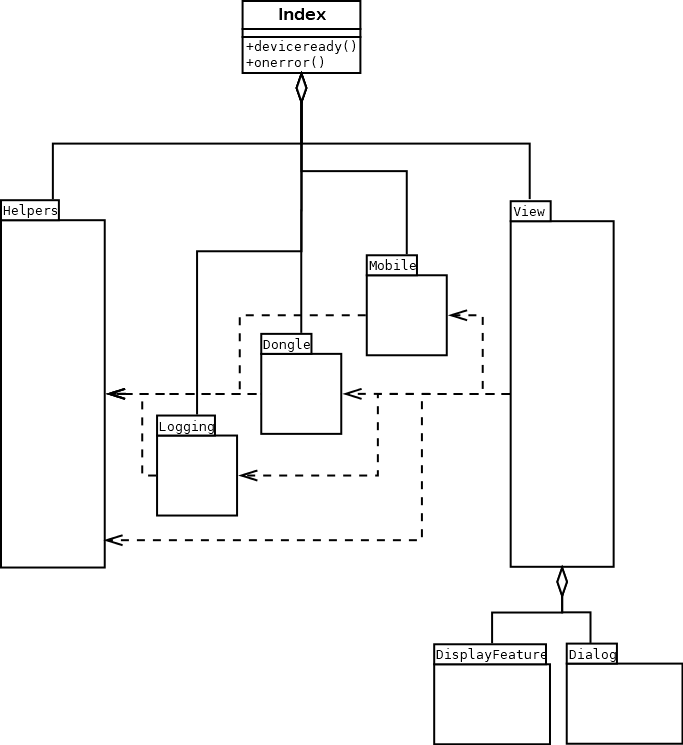
\includegraphics[width=8cm]{./img/App_Komponentendiagramm}
    \caption{TODO}
    \label{fig:appKomponentendiagramm}
  \end{center}
\end{wrapfigure}

\begin{figure}[h]
  \begin{center}
    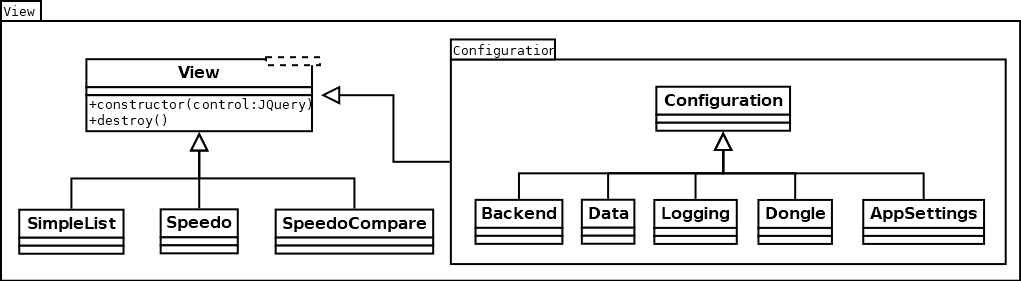
\includegraphics[width=\textwidth]{./img/App_Klassendiagramm_View}
    \caption{TODO}
    \label{fig:appKlassendiagrammView}
  \end{center}
\end{figure}

Hallo Welt 123

\begin{itemize}
\item Klassendiagramm (vllt mehrere mit Packet Diagramm)
\item Genereller aufbau (VSC-TS aufbau)
\item View prinzip
\item zusammenspiel mit displayfeatures und dialog
\item unterpunkt für configuration
\item zugriff auf Bluetooth (abstraktion über cordova framework)
\end{itemize}

\subsection{Buildsystem}
\begin{itemize}
\item Build System, Gulp files, zusammenfassen, optimieren , obfuscation von Dateien
\item Automatische generierung von Files wie variables.scss (nur sagen das sowas gemacht wird (wie steht in implementierung))
\item Embedden von images in scss (wie funktionierts und warum ist das wichtig)
\end{itemize}
\subsection{Testumgebung}
\begin{itemize}
\item Debug system im überblick (grober test im browser später auf vm und am schluss auf echten device mit debug möglichkeit über chrome) (nur grob später im Test bzw in Implementierung beschrieben) 
\end{itemize}



\section{Dongle}
\begin{sidewaysfigure}
  \begin{center}
    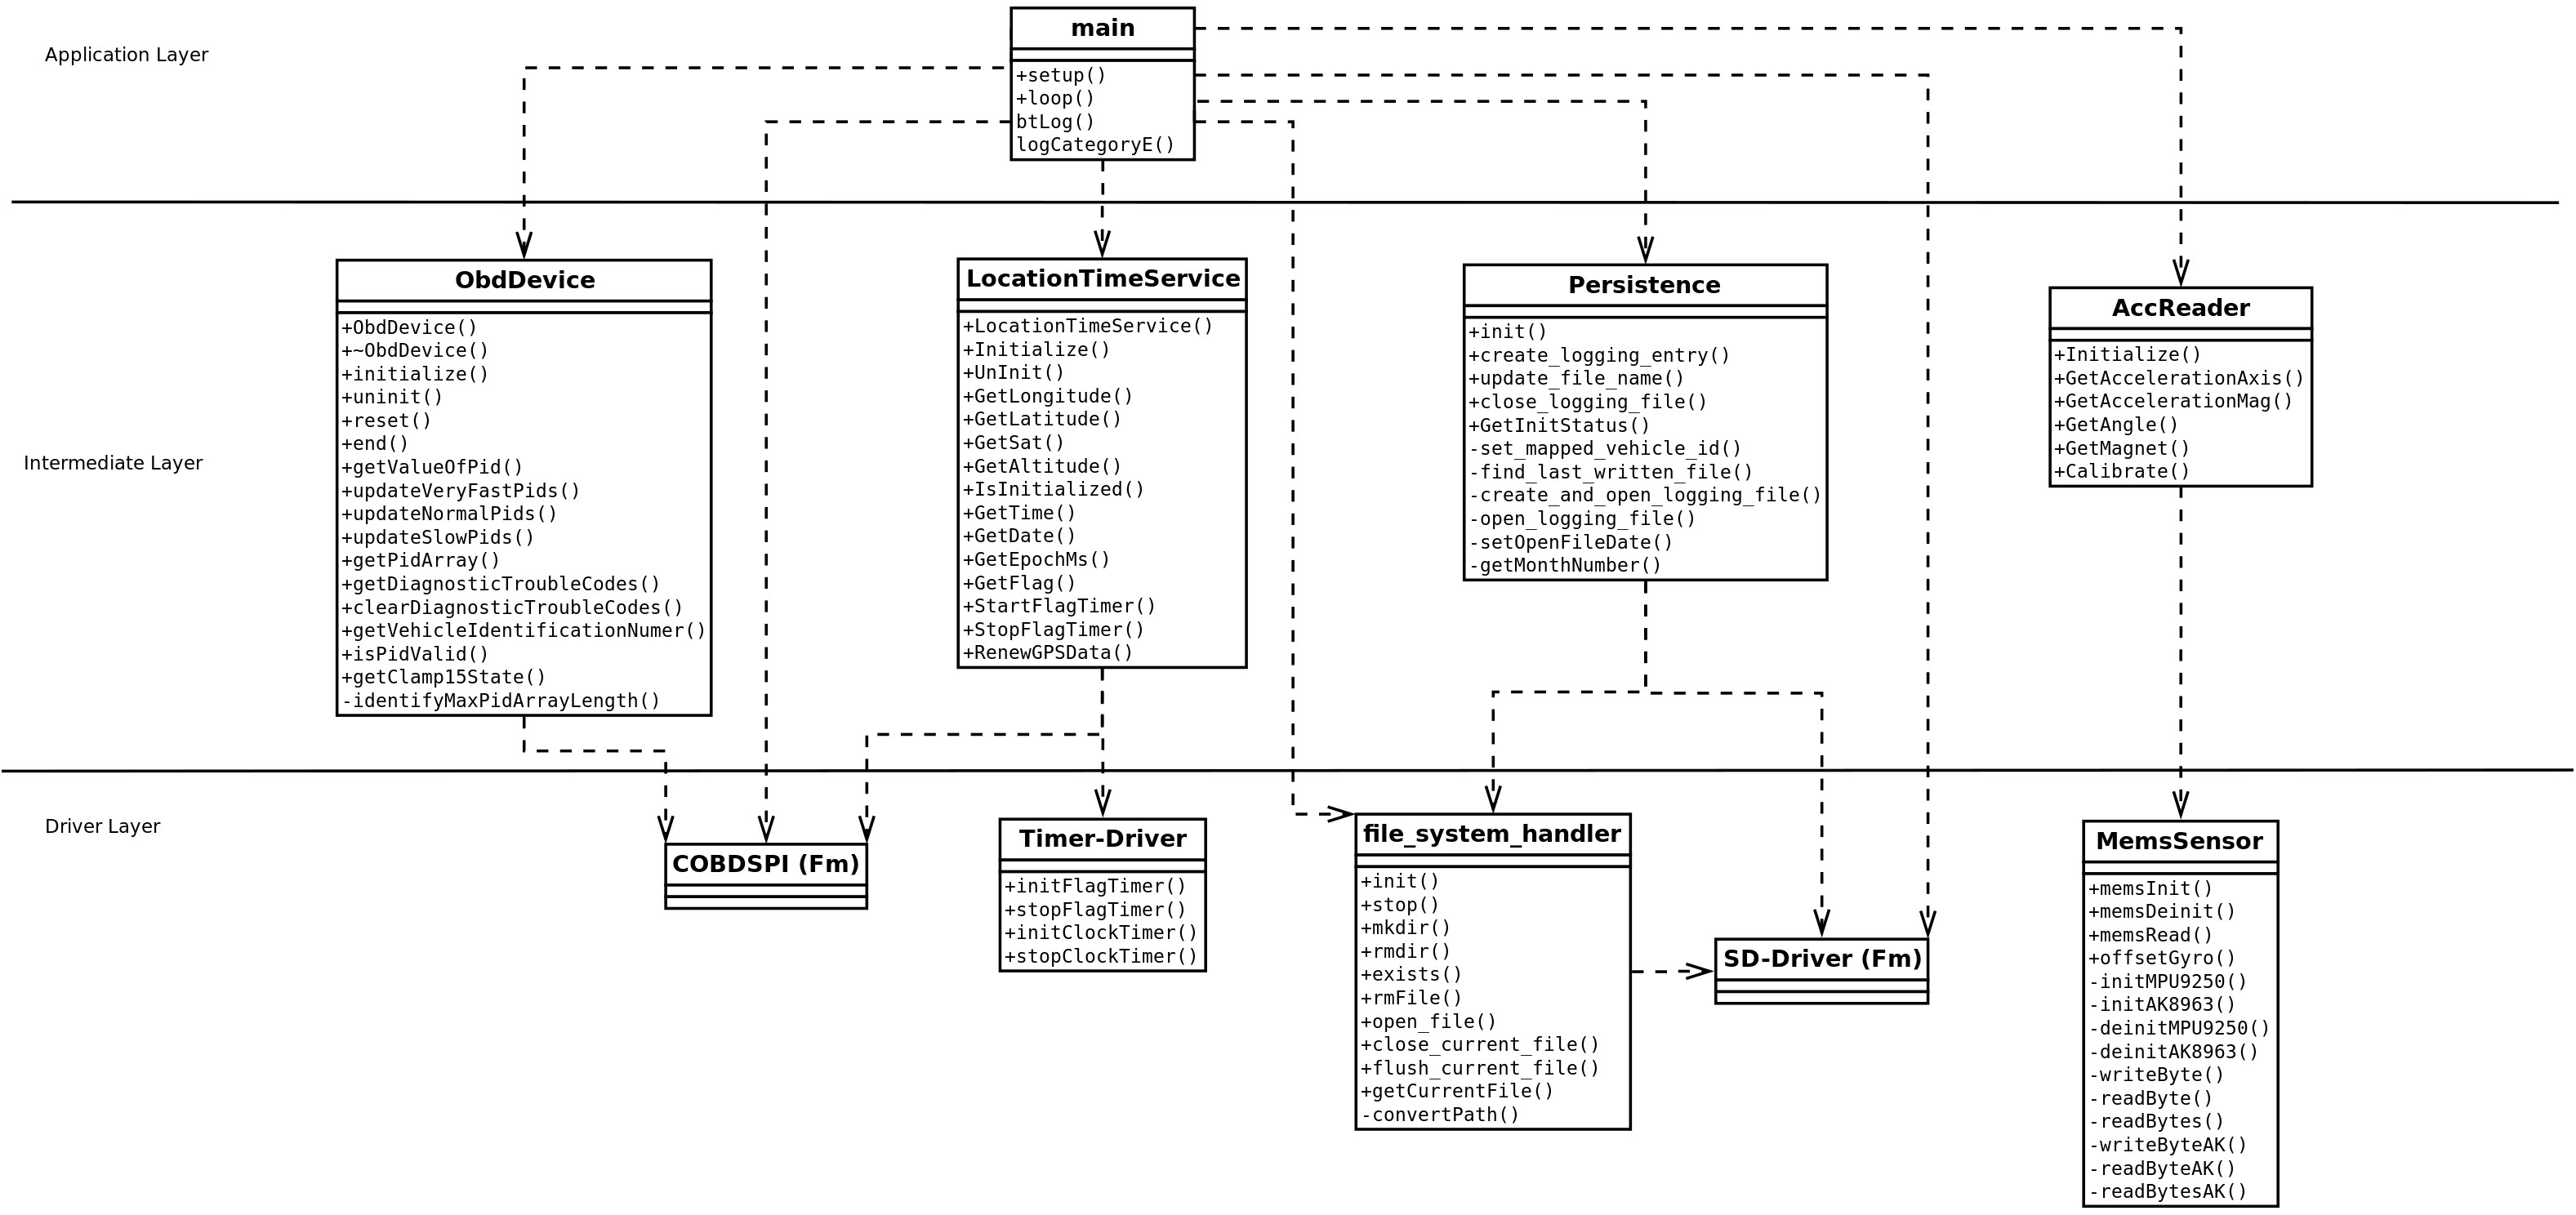
\includegraphics[width=\textwidth,height=15cm,keepaspectratio]{./img/Dongle_Arch_final}
    \caption{Architektur der Dongle-Software}
    \label{fig:dongleArch}
  \end{center}
\end{sidewaysfigure}
Um die Fahrzeugdaten gemäß den beschriebenen Use-Cases erfassen zu können, wurden mehrere Freematics ONE beschafft. Dieser Dongle bietet im Gegensatz zu manch anderen Adaptern die Möglichkeit Daten auf eine SD-Karte zu schreiben, mit Bluetooth zu kommunizieren und auf möglichst einfache Weise die darauf befindliche Software zu verändern. Wie auf der Produkthomepage beschrieben, nutzt der Dongle als Haupt-Controller einen ATmega328p, wie er auch auf einem Arduino UNO verwendet wird. Bei der Architektur der Dongle-Software wird deshalb für den Programmablauf ein für Arduino-Projekte klassischer Aufbau mit einer \enquote{setup}- und einer \enquote{loop}-Funktion innerhalb einer main-Datei verwendet.
\paragraph{}
Um bei der Entwicklung der Software für den Dongle möglichst wenig Inhaltsüber-schneidungen der Teammitglieder zu erreichen und um die Verständlichkeit und Wartbarkeit des Codes zu verbessern wurde entschieden die Schichtenarchitektur wie in Bild \ref{fig:dongleArch} umzusetzen.
Hierbei wird für die meisten Funktionsmerkmale mindestens eine Klasse auf der Intermediate-Layer sowie der Driver-Layer implementiert. Dies hat zur Folge, dass bei einer Funktionsänderung wie beispielsweise der Verwendung eines anderen GPS-Empfängers nur die entsprechende Treiber-Klasse geändert werden muss. Die Hauptklasse mit der eigentlichen Programmlogik bleibt dabei unangetastet.\\
Die im Bild \ref{fig:dongleArch} mit \enquote{(Fm)} ergänzten Klassen werden aus den Bibliotheken des Herstellers übernommen.
\subsection{GPS-Empfänger}
Da ein zentrales Ziel der Applikation die Anfertigung eines Fahrtenbuches mit Streckenaufzeichnung ist, muss auch die Position des Fahrzeuges möglichst genau bestimmt werden. Der in diesem Projekt verwendete Freematics ONE bietet hier die Möglichkeit, einen externen GPS-Empfänger über eine \ac{UART}-Schnittstelle anzubinden.
\paragraph{}
Um die Anschaffungskosten zu reduzieren, wurde zunächst untersucht, ob neben dem von Freematics verkauften GPS-Empfänger auch andere GPS-Receiver-Chips mit dem OBD-Dongle kompatibel sind.
Ein Problem bei dieser Untersuchung ist die Architektur des Freematics ONE, da die Kommunikation mit dem GPS-Empfänger nicht auf dem ATmega328p Haupt-Controller sondern auf einem STM32 Coprozessor ausgeführt wird. Leider ist der Code auf dem Coprozessor nicht öffentlich einsehbar und auch nicht ohne großen Aufwand auslesbar.
Ein weiteres Problem bestand darin, dass auch ein Öffnen des Gehäuses des von Freematics selbst vertriebenen GPS-Empfängers nicht zur Identifikation des Chips beitragen konnte. Es wurde allerdings klar, dass dieser nicht der Angabe auf der Produkthomepage des Freematics ONE entsprach. Der Empfänger-Chip ist nur mit einem QR-Code versehen und eine Recherche zum Hersteller verwies nur auf den chinesischen Produzenten des ganzen Empfänger-Moduls.(www.szgrltd.com)
\paragraph{}
Daher wurde eine andere Vorgehensweise zur Untersuchung der Kommunikation angewandt. Dazu wurde, wie in Abbildung \ref{fig:gpsAnalyse} abgebildet, ein zusätzlicher Arduino UNO als Zwischenstation in die UART-Kommunikation zwischen Dongle und Empfänger eingefügt. Zwei durch Software simulierte, serielle Schnittstellen auf dem Arduino UNO werden nun genutzt, um die vom Dongle und vom GPS-Empfänger gesendeten Daten aufzufangen, auf der über USB angeschlossenen seriellen Konsole eines Rechners auszugeben und an den jeweils anderen Kommunikationspartner weiterzuleiten.
\begin{figure}
  \begin{center}
    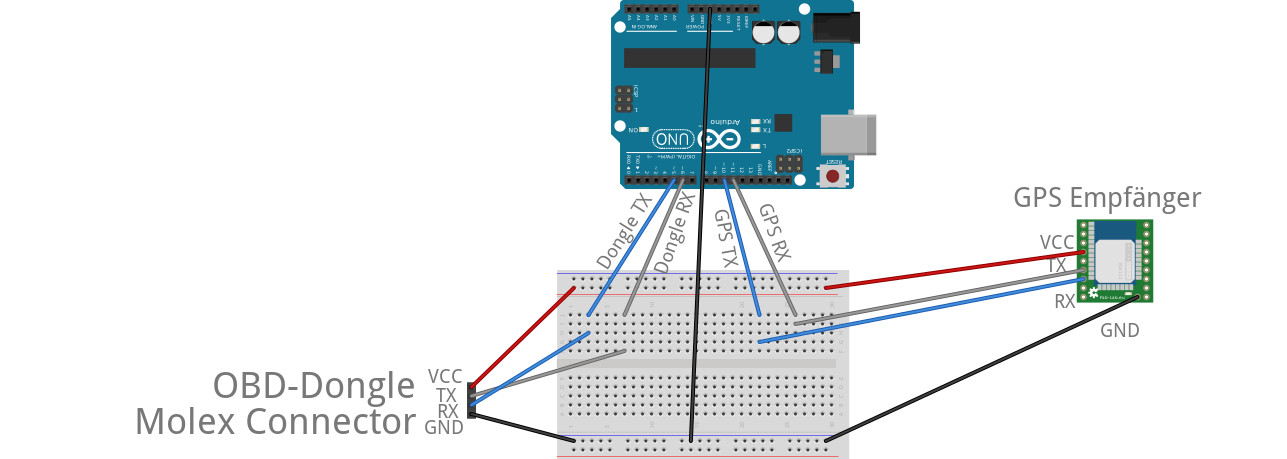
\includegraphics[width=\textwidth]{./img/gpsVersuch}
    \caption{Versuchsaufbau zur Analyse der UART-Kommunikation zwischen Dongle und GPS-Empfänger}
    \label{fig:gpsAnalyse}
  \end{center}
\end{figure}
\paragraph{}
Nach Auswertung der Kommunikation, stand fest, dass der von Freematics gelieferte GPS-Empfänger kompatibel zu einem u-blox UBX-G7020 ist. Dieser versendet standardmäßig Nachrichten gemäß dem \ac{NMEA} Standard. Darüber hinaus wurde ersichtlich, dass der OBD-Dongle keine Nachrichten zum GPS-Chip sendet.
\paragraph{}
Da nun allerdings der konkrete Empfänger feststand, konnte dazu die entsprechende Protocol Specification heruntergeladen und mit weiteren GPS-Empfängern verglichen werden.
Letztendlich wurde ein Pixhawk GPS Empfänger für einen Modellbau-Quadrokopter auf Basis eines u-blox Neo6M mit zusätzlichem Magnetfeld-Sensor ausgewählt. Dieser Mikrochip verfügt zwar nicht über die exakt gleiche Protocol Specification, die ab Werk konfigurierte Kommunikation jedoch ist nahezu identisch und kompatibel mit der des von Freematics gelieferten Produktes.
\paragraph{}
Um den neuen Empfänger am Dongle zu betreiben, wurde an dessen Signal-Eingängen ein 2x2-Molex Stecker passend angelötet. Die I2C-Pins des Magnetfeld-Sensors wurden dabei nicht belegt.
\paragraph{}
Ein erster Test mit der von Freematics bereitgestellten Software zeigte die grundsätzliche Funktion des neuen GPS-Moduls. Allerdings ist die Genauigkeit des Pixhawk-Empfängers etwas schlechter als die des UBX-G7020.

	\subsection{ \ac{OBD}-Schnittstelle}
		Da der Dongle vorwiegend genutzt werden soll um die \ac{OBD}-Daten (kurz \acp{PID}) aufzuzeichnen besitzt der Freematics ONE eine hierfür passende Schnittstelle. Bei den \acp{PID}\cite{OBD-2.net2018} handelt es sich um Daten die von bestimmten Sensoren (z.B. Drehzahl, Geschwindigkeit, Öl-Temperatur, ...) im Auto zu Verfügung gestellt werden.
		\ \\
		Bei \ac{OBD} handelt es sich um ein Protokoll welches nach dem \enquote{challenge-response}-Prinzip funktioniert. Dabei werden vom Client (Dongle) Anfragen an den Server (\ac{OBD}-Steuergerät im Auto) gesendet. Dieses antwortet anschließend mit den Werten des entsprechenden Sensors.
		\ \\
		Da es vom vorliegenden Auto abhängig ist, welche Steuergeräte verbaut sind und somit auch was für \acp{PID} unterstützt werden, ist es nicht bei jedem Auto möglich die selben Daten auszulesen.
		\ \\
		Da weiterhin der Platz auf dem Freematics ONE (sowohl RAM als auch Flash) sehr begrenzt ist, wurde von vorne herein entschieden, nur bestimmte \acp{PID} zu verwenden. Insgesamt wurden xy viele \acp{PID} ausgewählt. Um sowohl die \ac{OBD}-Schnittstelle als auch den Prozessor im Freeatics ONE unter wenig Last auszusetzen, dabei allerdings möglichst viel Nutzen aus den gewonnen Informationen ziehen zu können, wurden die \acp{PID} in unterschiedliche Gruppen eingeteilt. 
		\ \\
		Eine Gruppe entspricht somit einem Zusammenschluss aus \acp{PID} welche alle in einem gleichen Zeitintervall abgerufen werden. Es wurde sich für folgende Gruppen entschieden (Tabelle \ref{KategorieTable}):
		
		\begin{center}
			\begin{tabular}{|c|c|}
				\hline 
				Kategorie & Intervall \\ 
				\hline 
				A & 500ms \\ 
				\hline 
				B & 1,5s \\ 
				\hline 
				C & 15s \\ 
				\hline 
				D & 5min \\ 
				\hline 
				E & neue Route \\ 
				\hline 
				F & neues Auto \\ 
				\hline 
			\end{tabular} 
			\label{KategorieTable}		
		\end{center}

		
		Der Tabelle \ref{KategorieTable} kann zum einen entnommen werden, welche \acp{PID} ausgewählt wurden und in welcher Kategorie sie zugeordnet wurde.
		
		\begin{center}
			\begin{tabular}{|c|c|c|}
				\hline 
				Name & Wert & Kategorie \\ 
				\hline 
				Engine coolant temperature & 0x05 & C \\ 
				\hline 
				Engine RPM & 0x0C & A \\ 
				\hline 
				Vehicle speed & 0x0D & A \\ 
				\hline 
				Run time since engine start & 0x1F & C \\ 
				\hline 
				Distance traveled with malfunction indicator lamp & 0x21 & D \\ 
				\hline 
				Fuel tank level input & 0x2F & D \\ 
				\hline 
				Absolute barometric pressure & 0x33 & C \\ 
				\hline 
				Ambient ari temperature & 0x46 & C \\ 
				\hline 
				Fuel type & 0x51 & E \\ 
				\hline 
				Ethanol fuel \% & 0x52 & E \\ 
				\hline 
				Relative accelerator pedal position & 0x5A & A \\ 
				\hline 
				Engine oil temperature & 0x5C & C \\ 
				\hline 
				Engine fuel rate & 0x5E & A \\ 
				\hline 
				Driver's demand engine-percent torque & 0x61 & A \\ 
				\hline 
				Actual engine-percent torque & 0x62 & A \\ 
				\hline 
				Engine reference torque & 0x63 & A \\ 
				\hline 
				Engine run time & 0x7F & C \\ 
				\hline 
			\end{tabular} 
		\end{center}
		

\subsection{Zeit}
Wie bereits erwähnt, muss auch auf dem Dongle eine Repräsentation der genormten Zeit vorhanden sein. Zunächst soll jeder erfasste Datenwert mit einem Zeitstempel versehen werden um mit einer totalen Ordnung die Analyse dieser Werte erst zu ermöglichen. Zum anderen sollen die Datenwerte mit einem Intervall von 500 Millisekunden erfasst werden.
\paragraph{}
Die Anforderung nach einem genauen Zeitintervall von 500 Millisekunden zwischen dem Abrufen der OBD-Werte der Kategorie A kann durch den Einsatz eines Hardware-Timers und Interrupts gelöst werden.
Auf dem ATmega328p Hauptcontroller stehen dem Entwickler 3 Hardware-Timer zur Verfügung. Allerdings muss hierbei beachtet werden, dass die Arduino-Bibliothek den Timer 0 für die Funktionen delay() und millis() verwendet und dieser daher unangetastet bleiben sollte.\cite{arduinoTimer}
Da die Intervalle zum Abrufen der PID-Kategorien B, C und D ein Vielfaches der 500 Millisekunden der Kategorie A sind, müssen für diese keine weiteren Timer verwendet werden. Statt dessen kann ein einfacher Vergleich in Kombination mit dem Modulo-Operator genutzt werden (vgl. Abbildung \ref{fig:loop}).
\subsection{Beschleunigungssensor}
Zunächst wurde ermittelt, welcher Sensor im Dongle verbaut wurde. Anhand der Informationen auf der Produkthomepage sowie des Source-Codes des Treibers wurde ersichtlich, dass ein MPU-9250 \ac{MEMS}-Sensor mit jeweils 3 Achsen für Beschleunigungs-, Drehraten- und Magnetfeldmessung verbaut ist. Hierbei ist besonders, dass der Sensor für das Magnetfeld als I²C-Submodul am Sensor ausgeführt ist.
\subsection{Programmlogik}
\label{subsec:ProgLogik}
Die eigentliche Programmlogik kann wie bereits erwähnt in die Teile \enquote{Setup} und \enquote{Loop} getrennt werden.
\begin{figure}
  \begin{center}
    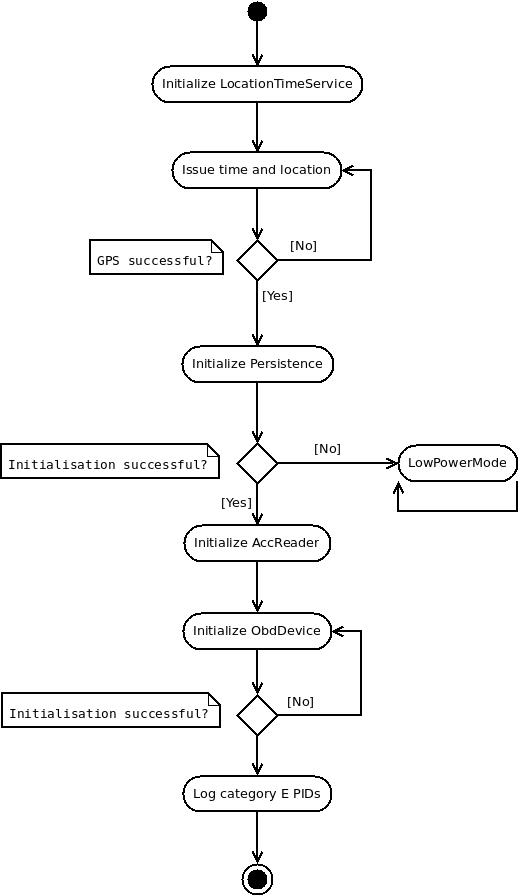
\includegraphics[width=\textwidth,height=10cm,keepaspectratio]{./img/Startup}
    \caption{Programmablauf der Initialisierung}
    \label{fig:setup}
  \end{center}
\end{figure}
\paragraph{}
Die Abbildung \ref{fig:setup} beschreibt den Ablauf des Programms beim Einstecken des Adapters in die Schnittstelle des Autos. Hervorzuheben ist, dass die Reihenfolge der Initialisierungen von großer Bedeutung ist. Näheres dazu wird im Kapitel \ref{subsec:intPl} erklärt.
\begin{figure}
  \begin{center}
    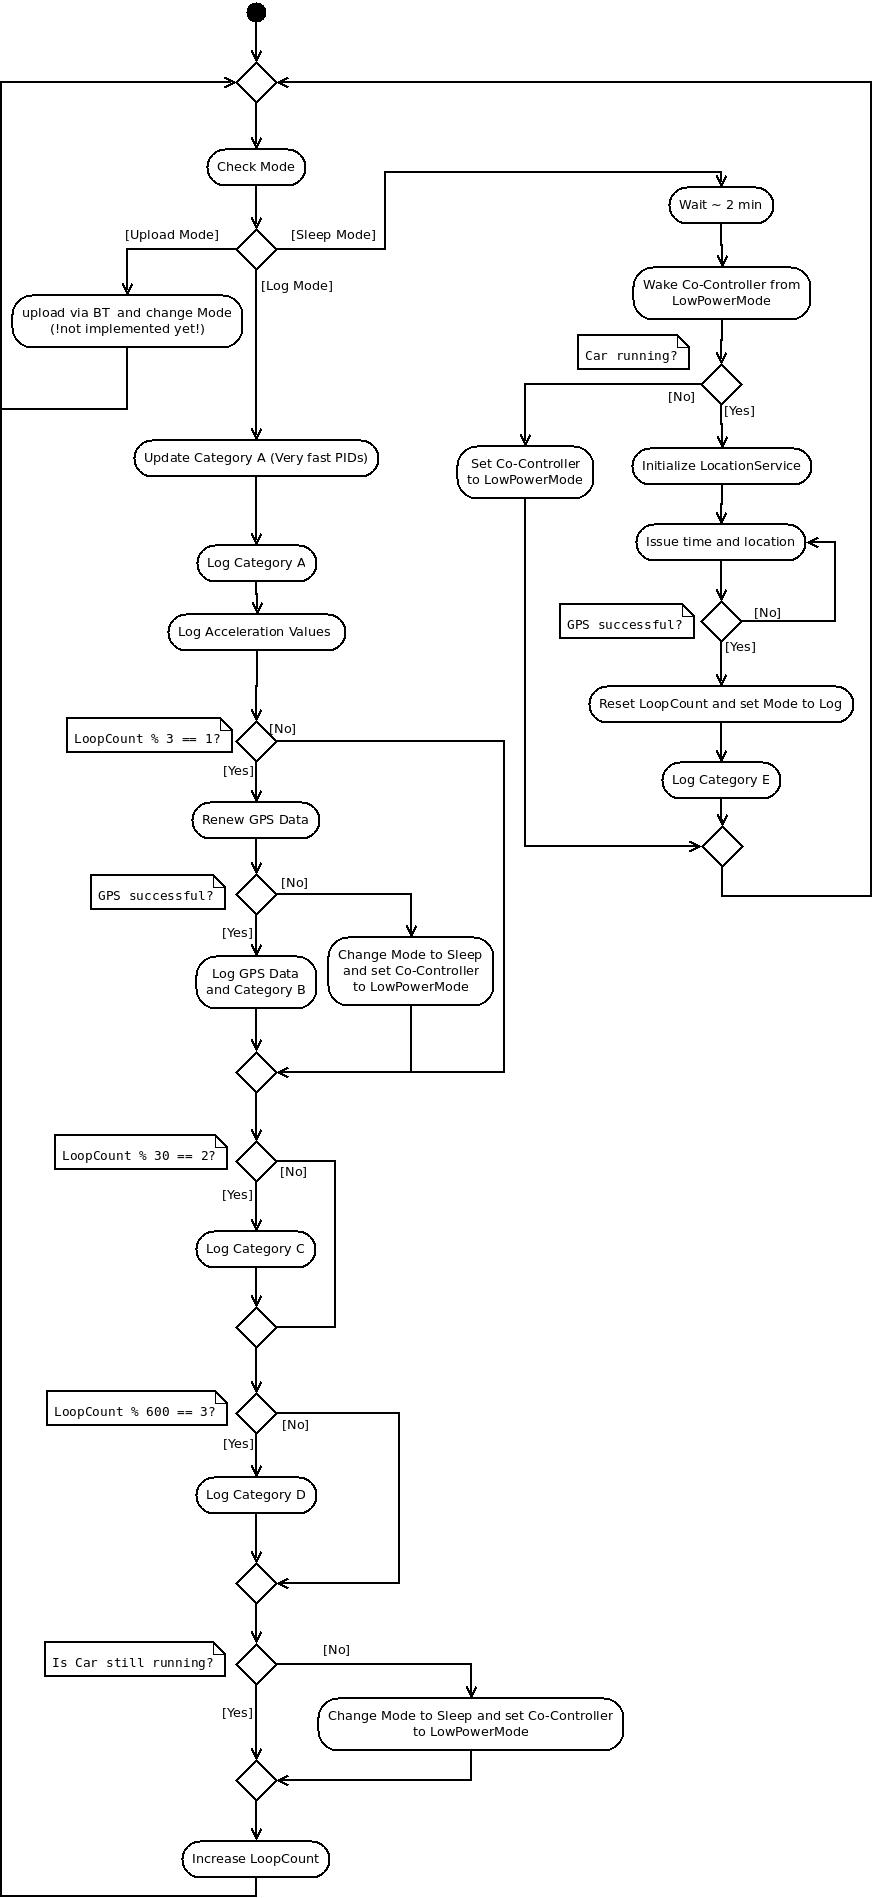
\includegraphics[width=\textwidth,height=20cm,keepaspectratio]{./img/ProgLoop}
    \caption{Programmablauf der Endlosschleife}
    \label{fig:loop}
  \end{center}
\end{figure}
In Abbildung \ref{fig:loop} ist der Ablauf des Programms ersichtlich, welches die eigentliche Funktionalität enthält. Dies wurde in drei Modi umgesetzt. Während des Logging-Modus werden die Fahrzeug-Daten gesammelt, auf eine SD-Karte geschrieben und per Bluetooth an ein Smartphone gesandt. Der Upload-Modus dient dazu, die gesammelten Daten auf der SD-Karte an die Smartphone-App weiterzugeben. Dies soll ein Entnehmen der Karte zum Auslesen der Daten optional machen. Der Schlafmodus dient letztendlich dazu, bei abgeschalteter Zündung das Bordnetz des Fahrzeugs möglichst wenig zu belasten.
